%!TeX root = ../complex_net_report_senacheribbe.tex
\graphicspath{{../assignment3/figures/}}

\subsection{Introduction and graph generation}

The objective of this third assignment is to generate and test the properties of a $G(n,p)$ graph. To generate it, we propose the \cref{algo:3}. Essentially for each node $i$, we add an edge to $n\_edges$ random previous nodes, with $n\_edges \sim Binomial(i, p)$. To tackle the fact we only add edges to previous nodes, the sparse matrix is finally added to its transposed version, obtaining an undirected graph.\\
The time complexity of this algorithm is $O(n+m)$, in opposition to the naive approach of sampling a random variable for each possible entry of the matrix (would be $O(n^2)$, too much for large $n$).

\begin{algorithm}[!ht]
	\caption{Generate $G(n,p)$}
	\label{algo:3}
	\begin{algorithmic}[1]
		\Function{generate\_gnp}{$n,p$}
		\State $graph \gets$ sparse matrix, size $n\times n$
		\\
		\For{$i = 0 \to n$}		
		\State $n\_edges \gets Binomial(i, p)$ 
		\If{$n\_edges > 0$}
		\State $choices \gets $ pick $n\_edges$ \textbf{random} elements from $0...i$ (no repetitions)
		\State $graph[i, choices]=1$
		\EndIf
		\EndFor
		\\	
		\State \Return $graph+transpose(graph)$
		\EndFunction
	\end{algorithmic}
\end{algorithm}

The sparsity of a $G(1000,0.1)$ is reported in \cref{fig:3_sparsity}. The sparsity of the matrix is uniform (we don't have gaps or recognizable structures) and the number of edges ($m = 49721$) is compatible with the expected number of edges we know from theory
\begin{equation}
\mathbf{E} (m)=\frac{n(n-1)p}{2}=49950
\end{equation}

\begin{figure} [!ht]
	\centering
	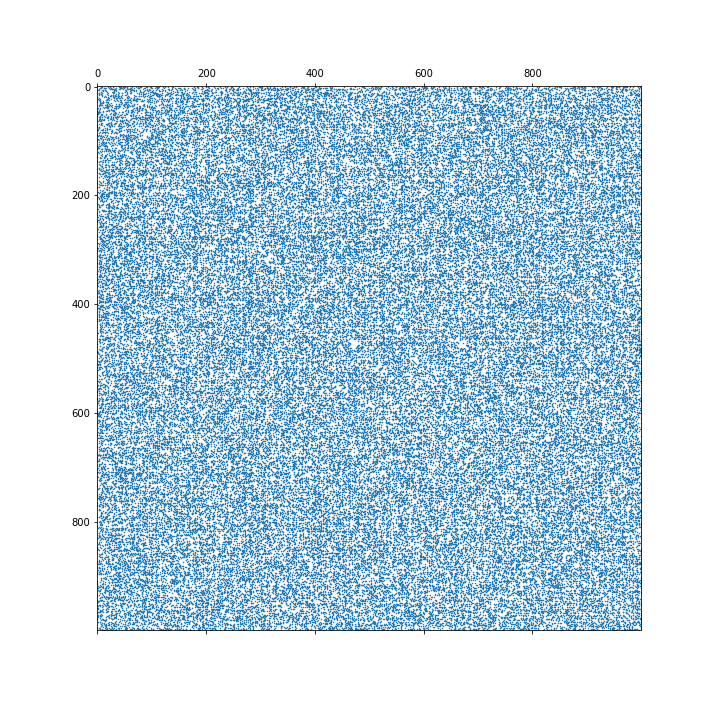
\includegraphics[width=.5\linewidth, clip, trim={2cm 2cm 2cm 2cm}]{sparsity}
	\caption{Sparsity of $G(n,p)$ with $n = 1000$ and $m = 49721$}
	\label{fig:3_sparsity}
\end{figure}


\subsection{Testing $G(n,p)$ properties}

To test the properties of the Erdős–Rényi model, we run several simulations varying both $n$ and $p(n)$. For each choice of the two parameters, $100$ simulations are performed and the results are averaged using a Monte Carlo approach.
The full set of results produced are reported in \cref{t:gnp}. Here we focus instead on the results for $n=100000$ (\cref{t:gnp_100000}), which is the largest $n$ we simulated (so more representative for an asymptotic analysis).
\pagebreak
\subsubsection{Distribution of node degree}
According to theory, the distribution of node degree should follow a binomial distribution (light tail). 
The minimum and maximum values of the node degree for all different $n$ and $p(n)$ are reported in \cref{t:gnp_100000}, while in \cref{fig:3_distr} the case $n = 100000$ and $p(n) = 2log(n)/n$ is shown.\\ As we can notice from the plot, the simulation fits perfectly a $Binomial(n-1, p)$.

\begin{figure} [!ht]
	\centering
	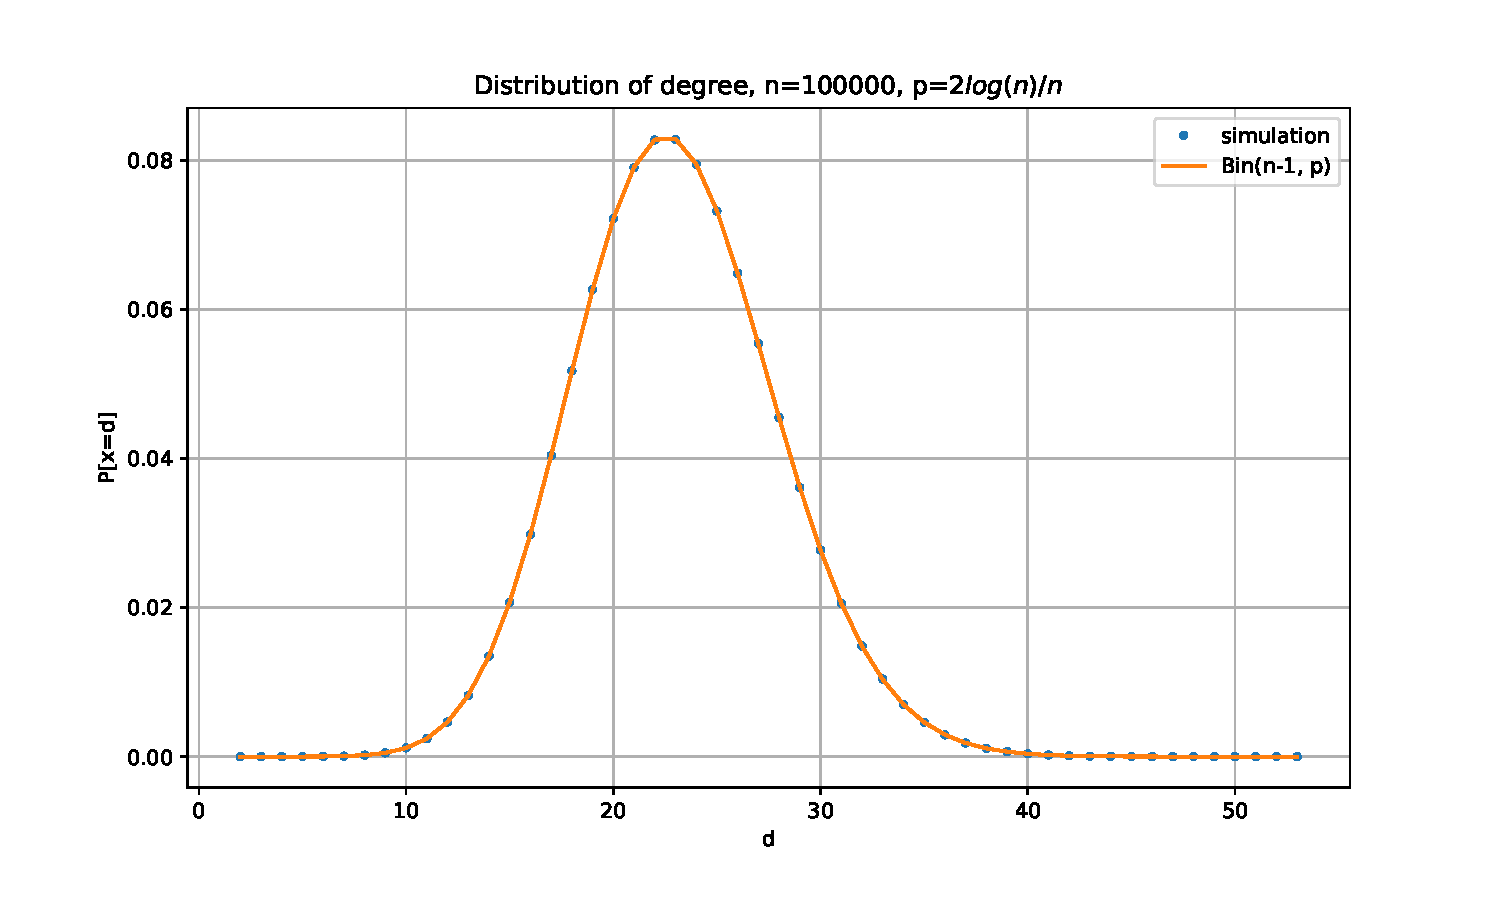
\includegraphics[width=.5\linewidth]{distribution}
	\caption{Distribution of degree $G(n,p)$ with $n = 100000$ and $p(n) = 2log(n)/n$}
	\label{fig:3_distr}
\end{figure}

\subsubsection{Diameter}
Calculating the exact diameter of a graph, ie the distance between the farthest nodes in the graph, is computationally expensive and not viable for large graphs like the one we are considering. We perform then an approximated calculation, which gives us a lower bound on the diameter. We sample randomly 20 nodes in the largest connected component and we compute the distance from them toward all the other nodes in the largest connected component.\\ The diameter is considered as the maximum distance found in this way. The results are reported in \cref{t:gnp_100000}. The first 2 rows should be excluded since the largest connected component is very small (we don't have a giant component). But from the third row, we can notice that $G(n,p)$ shows a small diameter ($\sim log(n)$), which decreases with increasing $p(n)$.

\subsubsection{Giant component}

The giant component is a connected component in which the number of nodes scales with $n$. To test its presence, we count the number of nodes in the largest connected component (\textit{1st cc}) and we consider it a giant component if it has at least $\frac{n}{10}$ nodes. In the column \textit{giant} of \cref{t:gnp_100000} we report the fraction of graphs that present this giant component (we run a Monte Carlo simulation with $100$ realisation for each $n$ and $p(n)$, 0 means none of the 100 graphs have this property, 1 all have it). \\
The transition from no giant to giant is abrupt between $0.9/n$ and $1.1/n$. As expected from theory, $1/n$ is a threshold function for the presence of the giant component. Moreover from the column \textit{2nd cc}, we can read the size of the second largest connected component. Again as expected from theory, when there is a giant component the 2nd connected component is a small component that scales at most with $log(n)$. The giant component is therefore unique.

\subsubsection{Connectivity}
Finally we analysed the connectivity of the graph. A graph is connected if there exists at least a path between any pair of nodes. Again from the table, we can notice that the graph is not connected up to the function $p(n)=0.9log(n)/n$ where we have a transition. $log(n)/n$ is a threshold function for the connectivity of the graph. We can also notice that approaching the threshold, the last nodes that remain outside the giant component and prevent the connectivity are isolated nodes (looking at \textit{2nd cc} we have it 1 for $0.9log(n)/n$ and $1.1 log(n)/n$).

\begin{table}[ht!]
	\centering
	\small
	\begin{tabular}{l|l|l|l|l|l|l|l}
		\toprule
		p(n) &  connected &  giant &  diameter &     1st cc &  2nd cc & deg\_min & deg\_max \\
		\midrule
		0.5/n &       0.00 &    0.0 &     12.55 &      25.90 &   22.47 &       0 &       8 \\
		0.9/n &       0.00 &    0.0 &     50.52 &     301.06 &  211.81 &       0 &       9 \\
		1.1/n &       0.00 &    1.0 &    160.08 &   17384.43 &  319.00 &       0 &      10 \\
		1.5/n &       0.00 &    1.0 &     52.59 &   58202.49 &   38.24 &       0 &      11 \\
		2/n &       0.00 &    1.0 &     31.90 &   79673.69 &   14.96 &       0 &      13 \\
		0.5 log(n)/n &       0.00 &    1.0 &     11.08 &   99678.32 &    2.02 &       0 &      22 \\
		0.9 log(n)/n &       0.03 &    1.0 &      7.60 &   99996.89 &    1.00 &       0 &      31 \\
		1.1 log(n)/n &       0.76 &    1.0 &      7.00 &   99999.74 &    1.00 &       0 &      38 \\
		1.5 log(n)/n &       1.00 &    1.0 &      6.00 &  100000.00 &     - &       1 &      44 \\
		2 log(n)/n &       1.00 &    1.0 &      5.00 &  100000.00 &     - &       2 &      54 \\
		0.01 &       1.00 &    1.0 &      3.00 &  100000.00 &     - &     153 &     490 \\
		\bottomrule
	\end{tabular}
\caption{Results from simulations of G(n,p), focus on $n=100000$}
\label{t:gnp_100000}
\end{table}

\begin{table}[ht!]
	\centering
	\small
	\begin{tabular}{l|l|l|l|l|l|l|l|l}
	\toprule
	n &          p(n) &  connected &  giant &  diameter &     1st cc &      2nd cc & deg\_min & deg\_max \\
	\midrule
	100 &         0.5/n &       0.00 &   0.05 &      3.89 &       5.90 &    4.310000 &       0 &       4 \\
	100 &         0.9/n &       0.00 &   0.71 &      8.07 &      14.88 &    7.990000 &       0 &       6 \\
	100 &         1.1/n &       0.00 &   0.92 &     11.76 &      27.47 &    9.270000 &       0 &       8 \\
	100 &         1.5/n &       0.00 &   1.00 &     15.03 &      53.39 &    7.190000 &       0 &       7 \\
	100 &           2/n &       0.00 &   1.00 &     13.68 &      78.19 &    3.710000 &       0 &       9 \\
	100 &  0.5 log(n)/n &       0.00 &   1.00 &     11.44 &      86.58 &    2.210000 &       0 &       9 \\
	100 &  0.9 log(n)/n &       0.21 &   1.00 &      6.69 &      98.46 &    1.050633 &       0 &      12 \\
	100 &  1.1 log(n)/n &       0.59 &   1.00 &      5.83 &      99.44 &    1.000000 &       0 &      14 \\
	100 &  1.5 log(n)/n &       0.85 &   1.00 &      4.43 &      99.84 &    1.000000 &       0 &      19 \\
	100 &    2 log(n)/n &       0.98 &   1.00 &      4.03 &      99.98 &    1.000000 &       0 &      23 \\
	100 &          0.01 &       0.00 &   0.82 &      9.34 &      19.72 &    8.430000 &       0 &       6 \\
	1000 &         0.5/n &       0.00 &   0.00 &      6.85 &      11.58 &    8.880000 &       0 &       5 \\
	1000 &         0.9/n &       0.00 &   0.09 &     19.13 &      56.58 &   28.490000 &       0 &       7 \\
	1000 &         1.1/n &       0.00 &   0.72 &     31.08 &     158.04 &   48.360000 &       0 &       8 \\
	1000 &         1.5/n &       0.00 &   1.00 &     30.76 &     579.34 &   14.720000 &       0 &       9 \\
	1000 &           2/n &       0.00 &   1.00 &     20.10 &     799.31 &    6.220000 &       0 &      10 \\
	1000 &  0.5 log(n)/n &       0.00 &   1.00 &     10.94 &     965.21 &    2.090000 &       0 &      14 \\
	1000 &  0.9 log(n)/n &       0.13 &   1.00 &      6.91 &     998.03 &    1.022989 &       0 &      18 \\
	1000 &  1.1 log(n)/n &       0.63 &   1.00 &      6.05 &     999.46 &    1.027027 &       0 &      21 \\
	1000 &  1.5 log(n)/n &       0.95 &   1.00 &      5.01 &     999.95 &    1.000000 &       0 &      29 \\
	1000 &    2 log(n)/n &       1.00 &   1.00 &      4.15 &    1000.00 &         - &       1 &      32 \\
	1000 &          0.01 &       0.96 &   1.00 &      5.04 &     999.96 &    1.000000 &       0 &      27 \\
	10000 &         0.5/n &       0.00 &   0.00 &      9.49 &      17.55 &   14.540000 &       0 &       7 \\
	10000 &         0.9/n &       0.00 &   0.00 &     30.81 &     134.35 &   89.460000 &       0 &       8 \\
	10000 &         1.1/n &       0.00 &   0.87 &     94.85 &    1676.05 &  169.850000 &       0 &       9 \\
	10000 &         1.5/n &       0.00 &   1.00 &     42.65 &    5825.63 &   24.420000 &       0 &      10 \\
	10000 &           2/n &       0.00 &   1.00 &     26.21 &    7967.78 &   10.300000 &       0 &      12 \\
	10000 &  0.5 log(n)/n &       0.00 &   1.00 &     10.90 &    9896.13 &    2.040000 &       0 &      18 \\
	10000 &  0.9 log(n)/n &       0.11 &   1.00 &      7.09 &    9997.51 &    1.000000 &       0 &      26 \\
	10000 &  1.1 log(n)/n &       0.71 &   1.00 &      6.18 &    9999.65 &    1.000000 &       0 &      30 \\
	10000 &  1.5 log(n)/n &       0.99 &   1.00 &      5.31 &    9999.99 &    1.000000 &       0 &      35 \\
	10000 &    2 log(n)/n &       1.00 &   1.00 &      5.00 &   10000.00 &         - &       2 &      42 \\
	10000 &          0.01 &       1.00 &   1.00 &      3.00 &   10000.00 &         - &      55 &     150 \\
	100000 &         0.5/n &       0.00 &   0.00 &     12.55 &      25.90 &   22.470000 &       0 &       8 \\
	100000 &         0.9/n &       0.00 &   0.00 &     50.52 &     301.06 &  211.810000 &       0 &       9 \\
	100000 &         1.1/n &       0.00 &   1.00 &    160.08 &   17384.43 &  319.000000 &       0 &      10 \\
	100000 &         1.5/n &       0.00 &   1.00 &     52.59 &   58202.49 &   38.240000 &       0 &      11 \\
	100000 &           2/n &       0.00 &   1.00 &     31.90 &   79673.69 &   14.960000 &       0 &      13 \\
	100000 &  0.5 log(n)/n &       0.00 &   1.00 &     11.08 &   99678.32 &    2.020000 &       0 &      22 \\
	100000 &  0.9 log(n)/n &       0.03 &   1.00 &      7.60 &   99996.89 &    1.000000 &       0 &      31 \\
	100000 &  1.1 log(n)/n &       0.76 &   1.00 &      7.00 &   99999.74 &    1.000000 &       0 &      38 \\
	100000 &  1.5 log(n)/n &       1.00 &   1.00 &      6.00 &  100000.00 &         - &       1 &      44 \\
	100000 &    2 log(n)/n &       1.00 &   1.00 &      5.00 &  100000.00 &         - &       2 &      54 \\
	100000 &          0.01 &       1.00 &   1.00 &      3.00 &  100000.00 &         - &     153 &     490 \\
	\bottomrule
\end{tabular}
\caption{Results from simulations of G(n,p)}
\label{t:gnp}
\end{table}